\chapter*{Aufgabenstellung}
\addcontentsline{toc}{chapter}{Aufgabenstellung}
%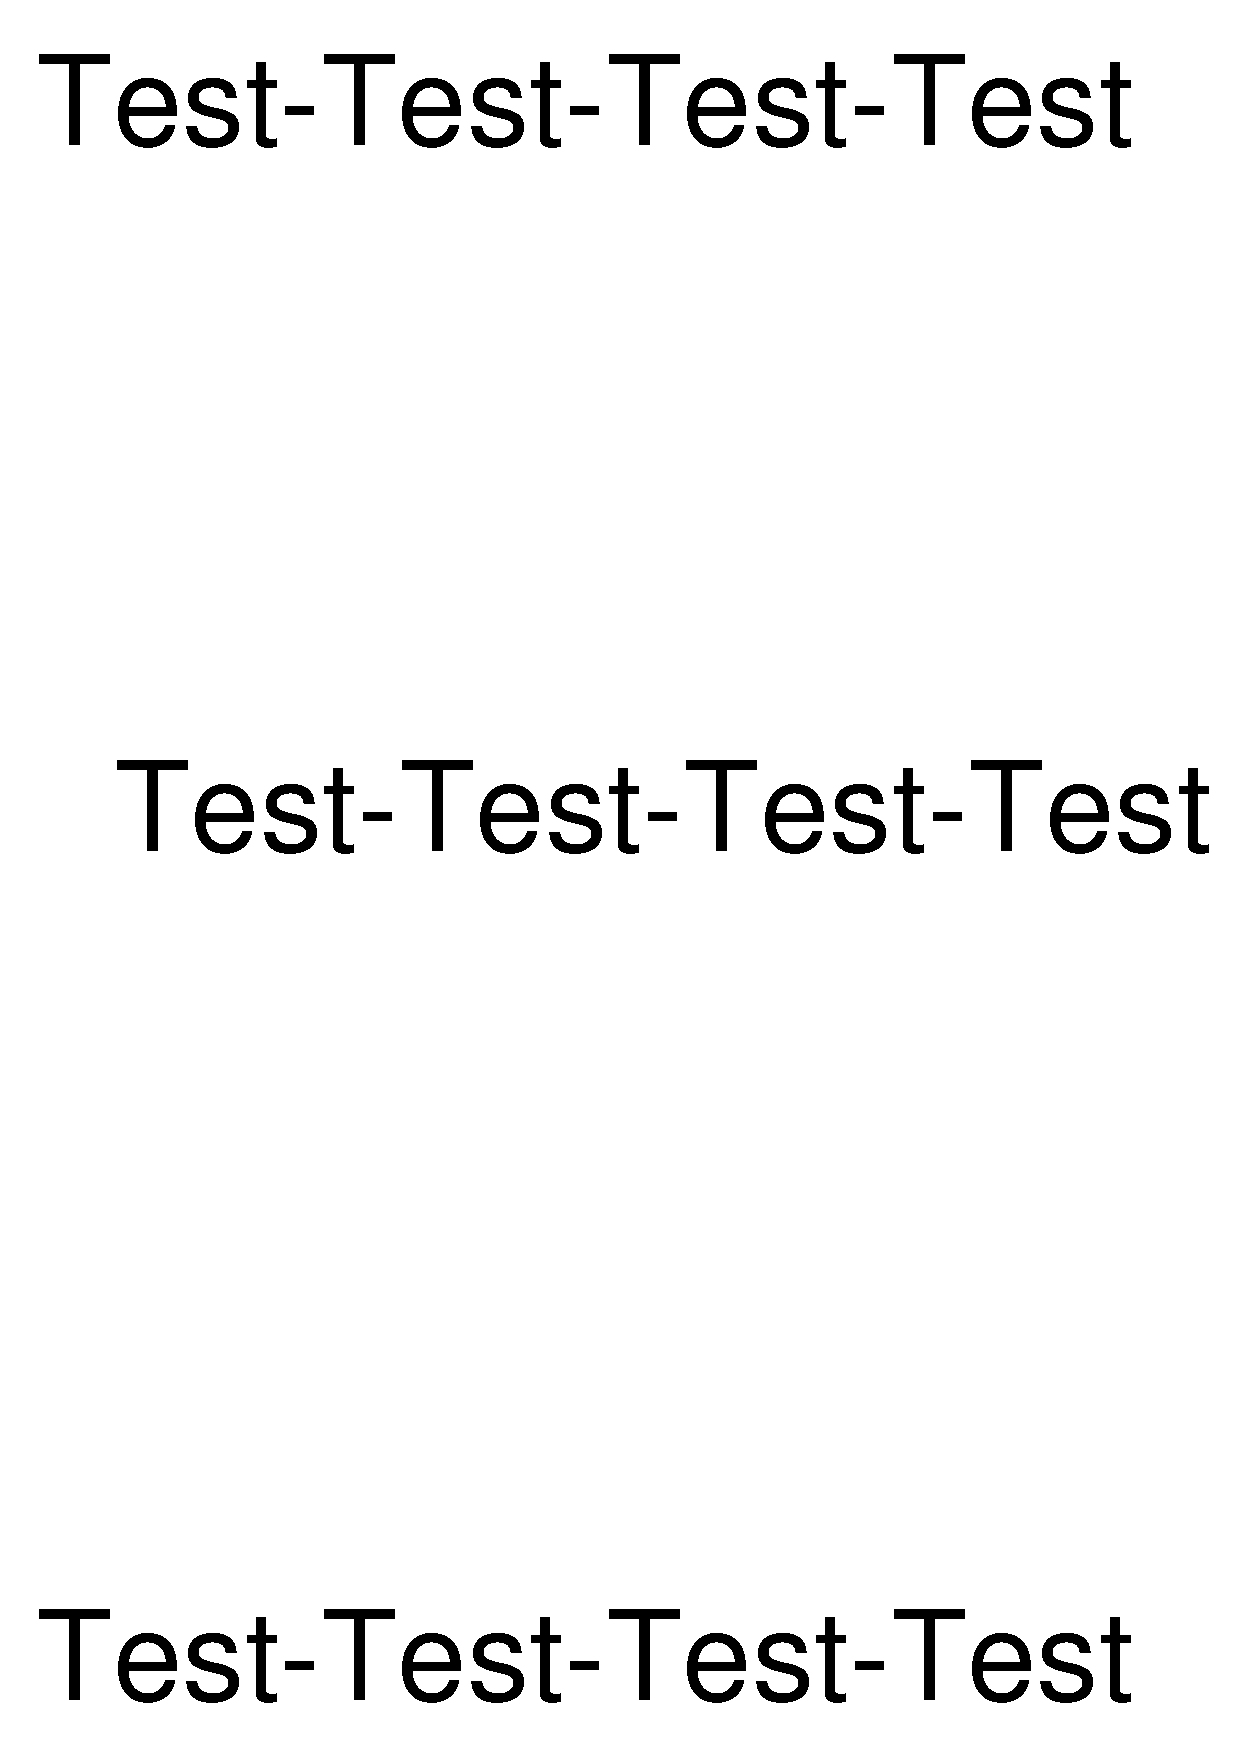
\includepdf[pages=1,scale=1,pagecommand={}]{include/Aufgabenblatt.pdf} %
\begin{enumerate}
    \item Messung des $\gamma$-Spektrums von $^{22}$Na, $^{137}$Cs und $^{57}$Co mit beiden Detektoren (NaJ-Detektor
    und Ge-Detektor). Energiekalibration mit Hilfe der Photopeaks.
    \item Messung des $\gamma$-Spektrums von $^{60}$Co mit beiden Detektoren. Bestimmung der Energie der Photolinien und Comptonkanten und Interpretation des Spektrums.
    \item Koinzidenzanalyse von $^{60}$Co mit unterschiedlichen Zeitschnitten. Welches Termschema beschreibt den Zerfall? Gibt es noch andere Koinzidenzen?
    \item Analyse der Abhängigkeit der Energieauflösung des Ge-Detektors und des NaJ-Detektors
    von der Energie. Wie lässt sich der Unterschied erklären?
\end{enumerate}